%--------------------------------------------------------------------------------
\documentclass[]{YIC2015}

% --------------------------------------------------------------------------------
% Include here your latex packages
%--------------------------------------------------------------------------------
\usepackage{graphicx}
\usepackage{color}
\usepackage{url}
\usepackage{subcaption}
% --------------------------------------------------------------------------------
% Article's title, with capital letter only at the beginning
%--------------------------------------------------------------------------------
\title{Modeling the I/O behavior of the NEST simulator using a proxy}

% -------------------------------------------------------------------------------
% List of authors
% --------------------------------------------------------------------------------
% Put the initials and surname of the first author ('et al.' if applicable) in
% square brackets before the command \author
%
% Identify the corresponding author with the command \corref and each author
% with the command \authref{a,b,...} according to the affiliation
%
\author[T. Schumann et al.]{%
  T. Schumann\authref{a}\corref,
  W. Frings\authref{b},
  A. Peyser\authref{c},
  W. Schenck\authref{c},
  K. Thust\authref{b},
  J.M. Eppler\authref{c}
}

% --------------------------------------------------------------------------------
% Affiliations
% --------------------------------------------------------------------------------
\address{\authaddr{a}{Institute of Neuroscience and Medicine (INM-6), Computational and Systems Neuroscience \\ %
    Institute for Advanced Simulation (IAS-6) \\ %
    J\"ulich Aachen Research Alliance \\ %
    Forschungszentrum J\"ulich GmbH \\ %
    52425 J\"ulich, Germany}
  \authaddr{b}{J\"ulich Supercomputing Centre \\ %
    Institute for Advanced Simulation \\ %
    Forschungszentrum J\"ulich GmbH\\ %
    52425 J\"ulich, Germany}
  \authaddr{c}{Simulation Lab Neuroscience - Bernstein Facility for Simulation and Database Technology \\ %
    Institute for Advanced Simulation \\ %
    J\"ulich Aachen Research Alliance \\ %
    Forschungszentrum J\"ulich GmbH \\ %
    52425 J\"ulich, Germany}
}
%
% --------------------------------------------------------------------------------
% Email address of the corresponding author
% --------------------------------------------------------------------------------
\corauth{till.schumann@rwth-aachen.de}

% --------------------------------------------------------------------------------
% Abstract
% --------------------------------------------------------------------------------
\abstract{\textit{ NEST \cite{NEST} is a simulator for spiking neural
    networks. It runs on ordinary desktop computers and notebooks,
    small clusters and supercomputers. Storing
    simulation data efficiently is essential for neuroscientific
    studies but is not trivial on supercomputers with centralized
    storage. To assess different I/O strategies and libraries, we have
    implemented a \emph{proxy} which imitates the writing behavior of
    NEST. This proxy is useful in benchmarking and statistical analysis, and
    thus consequent optimization, without the complexity of running
    full NEST simulations.}}

% --------------------------------------------------------------------------------
% Keywords - must be separated by semicolon and no capital letters.
% --------------------------------------------------------------------------------
\keywords{parallel I/O; simulation; neuronal networks; supercomputer;
  threading; MPI}

% --------------------------------------------------------------------------------
% Beginning of document
% --------------------------------------------------------------------------------
\begin{document}

\maketitle

% --------------------------------------------------------------------------------
% Beginning of one section
% --------------------------------------------------------------------------------
\section{Introduction}
%
Over the past 20 years, the NEST Initiative \cite{NESTInitiative} has
developed the NEST simulator \cite{NEST} for spiking neural network
models. It is used in computational neuroscience to simulate the
dynamics of interactions between nerve cells. The same code base is
used to simulate a range of networks, from small networks on local
machines up to large brain-scale circuits using the full capabilities
of the world's leading supercomputers. The basis of this flexibility
is a hybrid parallelization scheme using threads on a single node and
MPI \cite{mpi} to communicate between the compute nodes.

To record and store simulation data, NEST uses virtual recording
devices. One instance of each device (\emph{Spike detectors}
and \emph{Multimeters}) is created on each thread, and each instance
writes its data via a C++ stream to disk. For large-scale simulations
with many threads distributed over many compute nodes, this I/O
strategy fails, because of the large metadata overhead at the
filesystem level, e.g.~file creation alone can take up hours if a
supercomputer like JUQUEEN is fully used.

One solution used in recent releases of NEST has been the global spike
detector \cite{gsd}: a single file is opened by a dedicated MPI rank to
store spiking events, which is a low cost solution since all ranks
currently see all spike events through MPI collective communication.
On the other hand, the global spike detector has several long-term
consequences: 1) it constitutes a serialization bottleneck as spike
event I/O is handled by a single rank only without using all available
processors; 2) it is a design constraint, requiring all spikes being
globally available, which may not be scalable; and 3) it is
inapplicable to more voluminous data (e.g. membrane potentials) which
can not be tractably shipped to a single I/O node.

To overcome these problems, NEST requires an alternative approach to
file I/O. An important part of our efforts in this direction is the
specification and implementation of a \emph{NEST I/O proxy}, which
mimicks how NEST operates at the I/O level without actually executing
a full simulation. More specifically, it generates data writing
patterns similar to full NEST using fake data, avoiding a large part
of the computational costs of full NEST simulations during the
development and testing of new I/O backends. Using this proxy, we
have investigated possible performance gains by replacing the current I/O
paradigm with calls to parallelized I/O libraries which could avoid
serialization bottlenecks, thus paving the road for better I/O
performance in NEST.

\section{Design of the NEST I/O proxy}

To develop new I/O strategies, information about the writing behavior
of NEST is necessary. In order to get this information, the main
algorithms of NEST were analyzed and typical writing behavior was
statistically measured.

Given that NEST simulates an arbitrary neuronal network based on the
rules given in a simulation script, the program structure only gives
approximate and not exact information about the writing behavior. To
get the real runtime behavior, code analysis was accompanied by runtime
measurements for common use cases.

\subsection{Analysis of NEST code}

The main program structure of NEST can be reduced to an iteration loop
of gather, scatter and update functions of the network. Gather and
Scatter calls distribute the node states throughout the network. For
each node, the update function calls internal algorithms which process
the incoming information and update their state.

If the network node is a virtual recording device, the function called
depends on the type of incoming information. \emph{Spike detectors}
handle spike events and \emph{Multimeters} store internal parameters
of node objects. Whether or not a writing call occurs depends on the
neuronal network structure and activity.

\subsection{Measurements of runtime behavior}

To generate reliable timing measurements of the runtime behavior, part
of the NEST code (in particular the functions of the virtual recording
devices and their internal calls to lower-level I/O functions) were
manually instrumented with Score-P \cite{ScoreP}.
%
We have used the instrumented NEST binary to generate trace data for the
two use cases described in Sect.~\ref{sect:use_cases}.
From the trace data, we derived
statistical measures which describe the runtime behavior of NEST,
e.g.~the distribution of the onset of spike writing in each thread
relative to the start of the update phase in the main simulation cycle
of NEST.

\begin{table}[b]
\caption{Parameters which influence the I/O behavior of the proxy}
\centering
\begin{tabular}{lll}
\hline\hline
\textbf{Name}                   & \textbf{Type} & \textbf{Description} \\ \hline
numberOfSpikeDetectorsPerThread & Integer       & number of Spike detectors per thread  \\
numberOfMultimetersPerThread    & Integer       & number of Multimeters per thread  \\
spikesPerDetector               & Distribution  & number of spikes generated at each \\
        &           & Spike detector per iteration  \\
samplingIntervalsOfMeter        & Distribution  & sampling interval of the Multimeters  \\
numberOfValuesWrittenByMeter    & Distribution  & number of written values by each \\
        &           & Multimeter in sampling interval  \\
deadTimeUpdate                  & Distribution  & sleep timing between Spike detectors' \\
        &           & and Multimeters' write operations \\
deadTimeDeliver                 & Distribution  & sleep time in deliver function  \\
\hline\hline
\end{tabular}
\label{tab:table-silva1}
\caption{Input parameters for the NEST I/O proxy. The following distributions
  are implemented: Normal, Poisson, Binominal and fixed values.}
\end{table}

\subsection{Working principles of the proxy}

The NEST I/O proxy contains three main parts: Construction of the
network, the iteration loop and the destruction of the network. During
construction, each node creates the \emph{Spike detector} and
\emph{Multimeter} objects. Their numbers and properties are given by
the parameters shown in Table \ref{tab:table-silva1}. The iteration
loop contains a sleep function and update functions for the recording
devices. The sleep function is parameterized by the distribution
\emph{deadTimeDeliver}; the update functions execute a sleep function
parameterized by the distribution \emph{deadTimeUpdate}. During the
update function each \emph{Spike detector} or \emph{Multimeter} object
calls one or more write functions.

\begin{figure}[tb]
\centering %
\begin{subfigure}[b]{0.49\textwidth}
                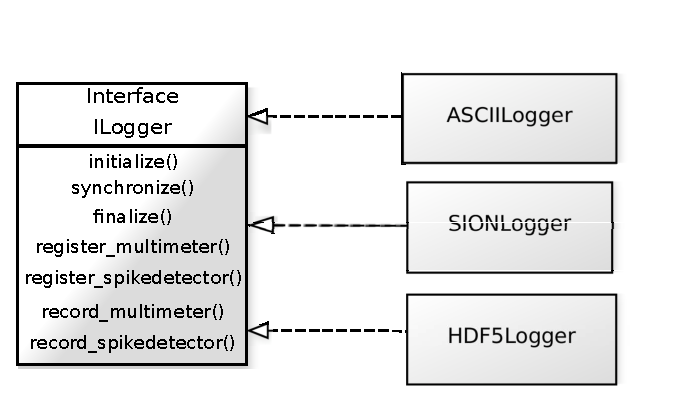
\includegraphics[width=.85\linewidth]{loggerinterface.eps}
                \caption{ILogger implements the I/O interface for the virtual
			recording devices.  Three differenct logger interfaces are
			available: \emph{ASCIILogger}, \emph{SIONLogger}, and
			\emph{HDF5Logger} (see section \ref{sec:io-drivers} for details). \cite{yuml}}
                \label{fig:loggerinterface}
        \end{subfigure}%
        \hspace{0.009\textwidth}
        \begin{subfigure}[b]{0.49\textwidth}
	      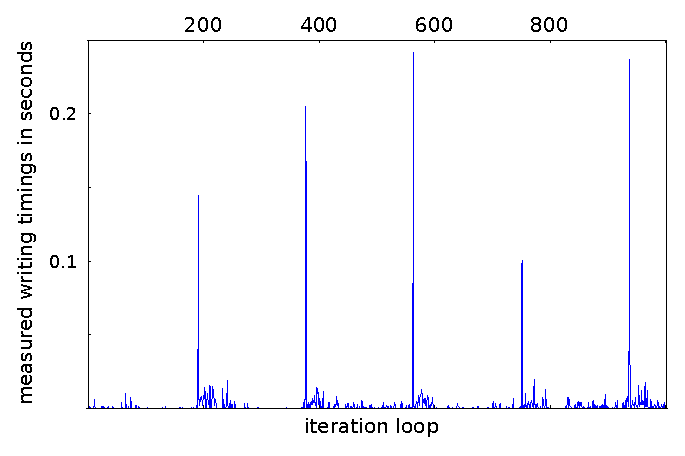
\includegraphics[width=.85\linewidth]{ascii_plot_10_8.eps}
	      \caption{NESTProxy output (used microcircuit model parametrization) plots the measured writing timings of the ASCII driver against internal iteration loop number.
	      \cite{yuml}}
	      \label{fig:asciiplot}
        \end{subfigure}%


\end{figure}

%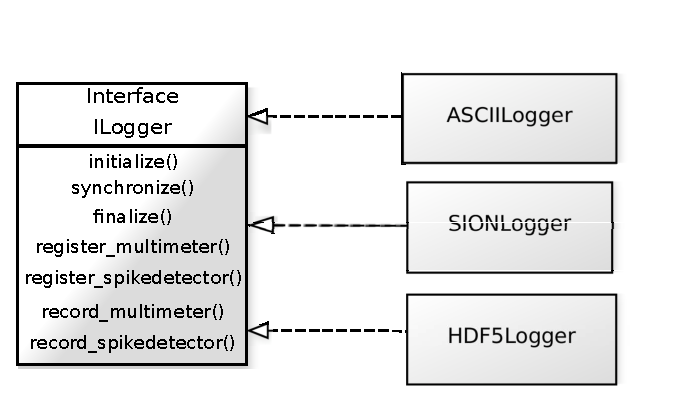
\includegraphics[scale=0.5]{loggerinterface.eps}
%\caption{ILogger implements the I/O interface for the virtual
%  recording devices.  Three differenct logger interfaces are
%  available: \emph{ASCIILogger}, \emph{SIONLogger}, and
%  \emph{HDF5Logger} (see section \ref{sec:io-drivers} for details). \cite{yuml}}
%\label{fig:loggerinterface}

\subsection{Basic I/O driver interface}

To provide maximum flexibility regarding the output format and to support all 
use cases of NEST, an interface (see Fig.~\ref{fig:loggerinterface})
has been developed to connect the virtual recording devices with different I/O 
libraries, allowing easy selection among them.


\section{Currently implemented I/O drivers}
\label{sec:io-drivers}

Based on the interface described above, three different drivers have been
implemented.

\paragraph{ASCII}

NEST currently uses C++ streams to store results as plain text files
containing time stamps as floating point strings. This scheme is
self-descriptive and simple to implement for post-processing and
analysis tools. However, this leads to excessive size of the data
stored to disk and serialization bottlenecks for metadata updates in
the file system when new blocks are allocated, in addition to the
problems described earlier regarding an excessive number of file open
operations leading to file system serialization. Nevertheless, We will
still used an ``ASCII'' driver as a benchmark against other
approaches, for debugging and validating other drivers, and as an
interface allowing backwards compatibility.

\paragraph{HDF5}

HDF5 is an API commonly used for file formats in the neuroscience
community such as NEO \cite{neo} and Neuroshare \cite{neuroshare}.
Since they use a common binary layout and API, data can be accessed
from many different languages and through many different libraries.
The HDF group publishes pHDF5 (parallel HDF5, \cite{hdf5}) which
allows read and write access to HDF5 files over MPI.

HDF5 is a highly structured, self-describing format intended for
long-term accessibility and versatile usage. This comes at the cost of
significant amounts of metadata to describe the data layout, creating
a collective barrier when finite data structures are extended. In
short, pHDF5 is read-oriented rather than write-oriented, with some of
the same drawbacks (and advantages) as the ASCII driver.

%For writing the data from large neuronal networks simulated in NEST,
%we have found it difficult to achieve a performance similar to what we
%got with SIONlib.

\paragraph{SIONlib}

SIONlib \cite{frings2009scalable} is a library which addresses most of
the common problems that arise from large scale parallel I/O. Its API
resembles task-local file I/O which makes it easy to replace the
existing ASCII driver in NEST.

Compared to HDF5, SIONlib's API is simpler since it does not describe
the data that is written, but only offers an interface for writing
byte steams, similar to ANSI-C. In general it focuses on performance
and simplicity and leaves the interpretation of the data to the user.

The most common write strategy in SIONlib is to only use collective
operations to open and close files; read and write calls are
independent and do not need any collective communication. This method
is highly scalable. Since it uses file system block alignment to
achieve better performance, it results in a significant amount of
unused space for scenarios where the volume of data per task is very
small, which is potentially the case for NEST. Hence for this case,
the collective writes in SIONlib are preferable.

\section{Benchmarking}

\subsection{Benchmark simulations}\label{sect:use_cases}

For benchmarking, we have used two typical simulation tasks: the
simulation of a random balanced network \cite{morrison07} and the
microcircuit model of a cubic millimeter of cortex \cite{potjans14}.
The first has very balanced I/O requirements while the latter is very
close to typical production runs carried out by the neuroscience
community.

To collect runtime data for the parametrization of the NEST I/O proxy,
we ran the random balanced network on a single compute node of the
supercomputer JUQUEEN split over 16 threads.  The simulation of the
microcircuit model was distributed over 32 compute nodes on JUQUEEN
with eight threads each; the overall number of neurons amounted to
80,000. Both \emph{Spike detectors} and \emph{Multimeters} were used
as recording devices.

\subsection{Results}

A final benchmark run shows the possibilities of the NESTProxy.  Using
the parametrization of a typical simulation (see
\ref{sect:use_cases}), we ran the NESTProxy using the current NEST
implementation of the ASCII driver.
%(1) The current ASCII implemenation from NEST, (2) a standard sionlib implementation and (3) a sionlib implemenations which buffers before writting.
The NESTProxy was executed on an Intel Xeon cluster using $10$ compute
nodes and $10$ threads per compute node. Mimicking the microcircuit
simulation described above with the NEST I/O proxy, we obtained the
benchmark results shown in Fig.~\ref{fig:asciiplot} for the current
ASCII driver implementation. The current NEST I/O \emph{ASCII}
implementation produces significant variation in writing timing.
Besides leading to large delays (up to $0.2$ seconds), this variation
also causes problems in workload optimization.

% \begin{itemize}
%   \item{Random balanced network: Dry-run simulation for M=32, T=16, N=300,000, mean firing frequ. of 7 Hz}
%   \item{Microcircuit model: Real simulation of only one area, run over 1000.0 ms: \\
% - Number of MPI processes: 32\\
% - Number of threads per MPI process: 8\\
% - Number of virtual processes (VPs): 256 (32x8)\\
% - Number of spike detectors per VP: 8\\
% - Number of neurons attached to each spike detector: 10000/256 (ca.)\\
% - Number of multimeters per VP: 8\\
% - Number of neurons attached to each multimeter: 500/256\\
% - MinDelay interval: Most likely equal to h step (= 0.1 ms)\\
% - Overall number of neurons in the network: 80,000}
% \end{itemize}

\section{Conclusions}

The NEST I/O proxy presented allows developers to flexibly switch
between several backends with different performance characteristics
and use-case profiles. It proved to be a useful tool in profiling and
benchmarking NEST's I/O over a range of parameters without the
computational and developmental overhead required to cover the same
range of possibilities using production runs of NEST.

Additionally, the proxy can be used as a generic tool for benchmarking
I/O strategies in general, given that NEST is a leading neuronal
network simulators with performance characteristics determined by the
same constraints which also affect similar software packages such as
NEURON \cite{neuron} and Brian \cite{brian}.

\section*{Acknowledgments}

Partially funded by the Helmholtz Association through the Helmholtz
Portfolio Theme "Supercomputing and Modeling for the Human Brain".
\pleasewrite{Till}{funded by the BBP of EPFL}


% --------------------------------------------------------------------------------
% Bibliography
% --------------------------------------------------------------------------------
\begin{thebibliography}{99}

\bibitem{NESTInitiative} NEST Initiative: The Neural Simulation
  Technology Initiative. \url{http://www.nest-initiative.org}.

\bibitem{NEST} %
  M.~Gewaltig, M.~Diesmann. NEST (NEural Simulation
  Tool). \textit{Scholarpedia} %
  \textbf{2.4}:1430, 2007.

\bibitem{gsd} S.~Kunkel et al. Spiking network simulation code for
  petascale computers.  \textit{Front.~Neuroinform.} \textbf{8}:78,
  2014.

\bibitem{ScoreP} Andreas Kn\"upfer et al. Score--P --- A Joint
  Performance Measurement Run--Time Infrastructure for Periscope,
  Scalasca, TAU, and Vampir. In: \textit{Proc.~of 5th Parallel Tools
    Workshop}, pp.~79--91, 2012.

\bibitem{neo} S.~Garcia et al. NEO: an object model for handling
  electrophysiology data in multiple formats.
  \textit{Front.~Neuroinform.}, \textbf{10}:8, 2014.
% \bibitem{neo} S.~Garcia, D.~Guarino, F.~Jaillet, T.~Jennings,
%   R.~Pr{\"o}pper, P.L.~Rautenberg, C.C.~Rodgers, A.~Sobolev,
%   T.~Wachtler, P.~Yger. NEO: an object model for handling
%   electrophysiology data in multiple formats.
%   \textit{Front.~Neuroinform.}, \textbf{10}:8, 2014.

\bibitem{neuroshare} The Neuroshare Project: Neuroshare Home
  Page. \url{http://neuroshare.sourceforge.net}.

\bibitem{hdf5} The HDF Group: HDF5 Home
  Page. \url{http://www.hdfgroup.org/HDF5/PHDF5}.

\bibitem{frings2009scalable} W.~Frings, F.~Wolf, V.~Petkov. Scalable
  massively parallel I/O to task-local files.  In: \textit{Proc.~of
  the Conference on High Performance Computing, Networking,
    Storage and Analysis}, article No.~17, 2009.

\bibitem{morrison07} A.~Morrison, A.~Aertsen,
  M.~Diesmann. Spike-timing-dependent plasticity in balanced random
  networks. \textit{Neural Computation} \textbf{19.6}:1437--1467,
  2007.

\bibitem{potjans14} T.C.~Potjans, M.~Diesmann. The cell-type specific
  cortical microcircuit: relating structure and activity in a
  full-scale spiking network model. \textit{Cereb.~Cortex}
  \textbf{24}:785--806, 2014.

\bibitem{neuron} M.~L.~Hines, N.~T.~Carnevale. The NEURON simulation
  environment. \textit{Neural Computation} \textbf{9.6}: 1179--1209,
  1997.

\bibitem{brian} D.~F.~M.~Goodman, R.~Brette. The Brian
  simulator. \textit{Front.~Neurosc.} \textbf{3.2}:192--197, 2009.
  
\bibitem{yuml} yUML: The diagram is generated by yUML. \url{http://yuml.me}

\bibitem{mpi} Message P Forum. Mpi: a Message-Passing Interface
  Standard. Technical Report. University of Tennessee, Knoxville, TN,
  USA. 1994.

\end{thebibliography}

\end{document}
